\section{Client boundary, data and assumptions}
The supplied generation portfolio and simulated wind farm form the client's
fixed starting assets \cite{brief}. Demand limits electricity sales. There
are no imports, extra export route or payment for unused power. Financial
results use repaired prices in constant 2020 pounds.

\begin{table}[H]
\centering\small
\caption{Input treatment. Replacements and estimate flags are recorded in the
cell-level audit \cite{repair}. Date counts overlap.}
\begin{tabularx}{\linewidth}{@{}M{.24\linewidth}Y@{}}
\toprule
Check & Treatment \\
\midrule
Calendar and totals & Align five series to 2,452 UTC days through
17 September 2026. Reconcile fuel output to total generation. \\
Daily statistics & Rebuild 7 generation, 350 demand and 346 price
query endpoints from full-day records. Daily mean MW is multiplied by 24 h. \\
Gaps and prices & Flag observed, interpolated and proxy values. Remove
zero-volume price records, volume-weight active providers, and use monthly CPI
to express prices in 2020 pounds \cite{cpi}. \\
\bottomrule
\end{tabularx}
\end{table}

Figure~\ref{fig:years} shows why 2023 is a useful low-surplus stress year:
it has the fewest surplus days and least surplus in the six complete years.
We also optimise a common equipment size over 2020--25 and replay it in each
year. These are historical evaluations using known daily conditions.
Partial 2026 results are retained in the calculation archive.

\begin{figure}[H]
\centering
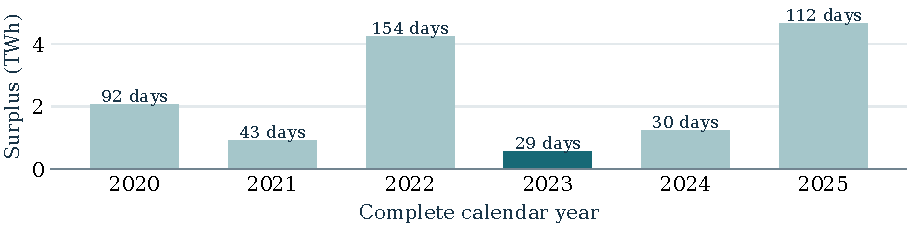
\includegraphics[width=.90\linewidth]{figures/annual_surplus.pdf}
\caption{Physical surplus and the number of positive-surplus days.
2023 is the lowest-surplus complete year. Source: repaired daily inputs.}
\label{fig:years}
\end{figure}

\begin{table}[H]
\centering\small
\caption{Reference technology and contract assumptions, in 2020 pounds.}
\begin{tabularx}{\linewidth}{@{}M{.16\linewidth}Y@{}}
\toprule
Input & Assumption and basis \\
\midrule
Battery & 1.5 MW / 3 MWh modules, 20--80\% state of charge, 90\% round-trip
efficiency, 15-year life. The brief's EUR 288,000/MWh becomes
\gbp 256,235/MWh. Fixed cost is \gbp 14,862/MW-year \cite{brief,dea,basis}. \\
Electrolyser & 20 MW modules, 20--100\% online load, 55.9 kWh/kg.
\gbp\Capital m installed per module, \gbp 0.52m/year fixed cost,
30-year life and \gbp 9.79m renewals in years 11 and 22 \cite{iea,beis,basis}. \\
Finance and buyer & 5\% real discount, \gbp\Netback/kg netback after
non-power variable costs, and a 10 t/day buyer cap. The cap and discount
rate are modelling assumptions. \\
\bottomrule
\end{tabularx}
\end{table}

\samplebreak
\section{Investment model and comparison}
\subsection{Formulation}
For day \(t\in\mathcal T\), \(G_t,D_t\) are supply and demand (MWh),
\(p_t\) is price (\gbp/MWh), \(v\) hydrogen netback (\gbp/kg) and
\(L\) offtake (kg/day). Decisions \(q_t,c_t,r_t,h_t,u_t\) are direct sale,
charge, discharge, electrolysis input and unused generation (MWh).
Installed \(b,n\) and online \(z_t\) are module counts.
\(\kappa=0.0559\) MWh/kg. Represented years \(Y\) equal one for a complete
year, six for 2020--25 and \(280/365\) for the strict 2023 subset.

\begin{subequations}\label{eq:model}
\begin{align}
\max\quad & \frac{1}{Y}\sum_{t\in\mathcal T}
\left[p_t(q_t+r_t)+v h_t/\kappa\right]-a_Bb-a_Hn,\label{eq:obj}\\
\text{subject to}\quad
&q_t+c_t+h_t+u_t=G_t,\qquad q_t+r_t\le D_t,\label{eq:balance}\\
&c_t\le E_Bb/\eta,\quad r_t\le\eta E_Bb,\quad
\sum_t r_t=\eta^2\sum_t c_t,\label{eq:battery}\\
&E_H^{\min}z_t\le h_t\le E_H^{\max}z_t,\quad h_t/\kappa\le L,
\quad z_t\le n,\label{eq:h2}\\
&q_t,c_t,r_t,h_t,u_t\ge0,\qquad b,n,z_t\in\mathbb Z_{\ge0}.\label{eq:domain}
\end{align}
\end{subequations}

The day-indexed constraints hold for every \(t\). Equation~\eqref{eq:balance}
allocates generation and limits sales. Equation~\eqref{eq:battery} gives one
usable daily window, \(E_B=1.8\) MWh per battery, with
\(\eta=\sqrt{0.90}\), and balances storage over the sample.
In \eqref{eq:h2}, \(E_H^{\min}=96\) and \(E_H^{\max}=480\) MWh
bound online loading and \(L\) limits hydrogen sales.
Policy A freely allocates power by value. Policy B also fixes
\(q_t=\min(G_t,D_t)\); it sells even at negative prices.

Equivalent annual cost for asset \(j\in\{B,H\}\) is
\begin{equation}
a_j=F_j+\frac{i}{1-(1+i)^{-N_j}}
\left(K_j+\sum_{k\in\mathcal R_j}\frac{C_{jk}}{(1+i)^k}\right).
\label{eq:eac}
\end{equation}
Here \(F_j,K_j,N_j,i\) are annual fixed cost, initial cost including
commissioning, life and discount rate. \(\mathcal R_j\) lists renewal years
with cost \(C_{jk}\). Gains use the same-policy zero-investment comparator;
the code subtracts its constant revenue to resolve small investment differences.

\subsection{Reference-year portfolios and matched strategy}
Table~\ref{tab:portfolios} shows the 2023 stress-year result. The same
20 MW asset under a sale-first rule captures the same \Capture~GWh of surplus
but loses \gbp\SimpleLoss m/year. A earns \gbp\RuleAdvantage m/year more
by also diverting saleable electricity. No additional foresight is needed for
this no-battery comparison: both use that day's inputs.
\begin{table}[H]
\centering\small
\caption{2023 capacity (battery / electrolyser MW) and gain (\gbp m/year) under the same-policy comparator.}
\label{tab:portfolios}
\begin{tabularx}{\linewidth}{@{}Y r r r r@{}}
\toprule
Scenario & A capacity & A gain & B capacity & B gain \\
\midrule
No investment & 0 / 0 & 0.00 & 0 / 0 & 0.00 \\
Battery only & 0 / 0 & 0.00 & 0 / 0 & 0.00 \\
Hydrogen only & 0 / 20 & 8.57 & 0 / 0 & 0.00 \\
Joint choice & 0 / 20 & 8.57 & 0 / 0 & 0.00 \\
Fixed 20 MW & 0 / 20 & 8.57 & 0 / 20 & \negval{1.07} \\
\bottomrule
\end{tabularx}
\end{table}


Across the complete six-year sample, a common 20 MW size is optimal under
both policies. Average incremental values are \gbp\MeanA m/year in A and
\gbp\MeanB m/year in B. The B outcome depends on the available surplus
in each year, as Table~\ref{tab:years} shows.

The supported benchmark (\gbp 175/MWh, 2012 pounds) becomes
\gbp\Netback/kg using 39.4 kWh/kg and CPI. We treat this as realised netback
with no further non-power deduction, in place of the brief's \gbp 9.50/kg.
Capital uses the IEA installed midpoint; fixed and stack costs use separate
UK reference estimates \cite{har,iea,beis,basis}.

\samplebreak
\section{What changes the investment decision?}
\subsection{Energy capture and the buyer constraint}
Physical surplus is \(S_t=\max(G_t-D_t,0)\).
In 2023, unused generation falls from \Surplus~GWh to \Unused~GWh.
The 20 MW electrolyser uses \Hinput~GWh: \Capture~GWh of surplus and
\Displaced~GWh diverted from direct sale. Surplus is \CaptureShare\% of
input and the plant captures \SurplusShare\% of annual surplus.
All 29 surplus days use the full 0.48 GWh/module. At 10 t/day, the buyer
can accept at most 0.559 GWh/day of electrolysis input; larger equipment
could therefore capture at most \PhysicalCap~GWh of that year's surplus.

With no battery and surplus-first attribution, \(C_t=\min(h_t,S_t)\).
If \(R_t\) is wind and solar output, their contribution \(W_t\) to capture obeys
\begin{equation}
\max(0,C_t-(G_t-R_t))\le W_t\le\min(C_t,R_t).
\end{equation}
The annual interval is 0--\Capture~GWh. Adding biomass and run-of-river
hydro to the renewable definition leaves this interval unchanged.
The aggregate fuel data do not identify the captured source.

\subsection{Contract thresholds and retained electricity sales}
At 10 t/day, the 20 MW break-even is \gbp\BreakA/kg in 2023 A and
\gbp\BreakB/kg in B. At \gbp\Netback/kg, A first breaks even at
\OfftakeBreak~t/day acceptance; \gbp\RefGain m/year corresponds to the
10 t/day reference contract. At that cap, doubling equipment to 40 MW
reduces annual gain to \gbp\FortyGain m. With 50 t/day, A selects
120 MW and gains \gbp\ExpansionGain m/year on \gbp\ExpansionCapital m capital.

\begin{figure}[H]
\centering
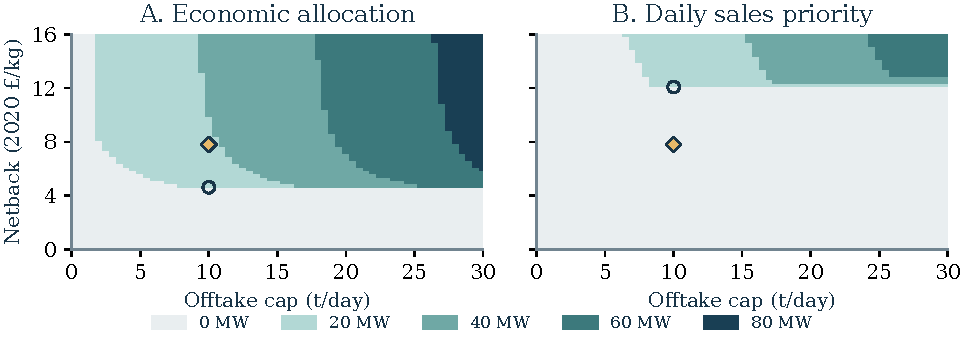
\includegraphics[width=\linewidth]{figures/contract_trigger.pdf}
\caption{Optimal 2023 capacity. Diamonds are the reference terms; open circles
show the fixed 20 MW break-even at 10 t/day. Values after non-power variable costs.}
\label{fig:contract}
\end{figure}

The following annual floors let the operator choose which sales to preserve,
relative to 215.1 TWh sold without investment. The 99.99\% floor binds.
Policy B instead gives electricity priority each day.
\begin{table}[H]
\centering\small
\caption{Realised sales lost and investment under annual floors, 2023 A.}
\label{tab:floors}
\begin{tabularx}{\linewidth}{@{}Y r r r@{}}
\toprule
Annual rule & Lost sales (GWh) & H$_2$ (MW) & Gain (\gbp m/year) \\
\midrule
A without floor & 157.9 & 20 & 8.57 \\
Restore half the sales loss & 79.0 & 20 & 5.19 \\
Retain 99.99\% of sales & 21.5 & 20 & 1.04 \\
Retain all sales & 0.0 & 0 & 0.00 \\
\bottomrule
\end{tabularx}
\end{table}


\paragraph{Verification.}
All \CheckCount{} Xpress schedules reconcile flow and cash; physical residuals
are below 0.001 MWh. Eight contract points match enumeration. All 14 annual
replays match the independent implementation's published precision \cite{peer}.

\samplebreak
\section{Historical performance and investment conditions}
\begin{table}[H]
\centering\small
\caption{Fixed 20 MW on all complete years. Gains are \gbp m/year under each policy; dispatch uses realised daily inputs.}
\label{tab:years}
\begin{tabularx}{\linewidth}{@{}Y r r r@{}}
\toprule
Year & Surplus (GWh) & A gain & B gain \\
\midrule
2020 & 2067 & 16.78 & 3.12 \\
2021 & 911 & 6.29 & \negval{0.13} \\
2022 & 4240 & 8.91 & 7.31 \\
2023 & 550 & 8.57 & \negval{1.07} \\
2024 & 1229 & 11.95 & \negval{1.00} \\
2025 & 4660 & 13.17 & 4.48 \\
2020--25 mean & 2276 & 10.94 & 2.12 \\
\bottomrule
\end{tabularx}
\end{table}

2023 is a surplus stress case, while 2021 is A's weakest complete year.
The positive B mean includes three losing years; a historical average
requires the client to tolerate that variation. In the 2025 joint downside
of \gbp 4/kg and 5 t/day, both policies lose money. A's 2023 gain is still
\gbp\CostStress m/year when initial installation costs rise 25\% and the
real discount rate becomes 8\%, holding stack cost fixed.
The strict-quality 2023 subset retains the original capacities.

\paragraph{Battery and model checks.}
The six-year free-charge revenue ceiling is \gbp\BatteryBound k/module-year,
below the \gbp\BatteryCost k annual cost, ruling out battery investment
in that common-size appraisal. For one fixed battery in 2023 A,
the annual pool gives \gbp\PoolValue k operating value; chronological
stock gives \gbp\StockValue k, with
\(s_t=s_{t-1}+\eta c_t-r_t/\eta\), \(0\le s_t\le E_Bb\) and zero
initial and terminal usable stock.

\begin{table}[H]
\centering\small
\caption{2023 A cash and annual-value bridge for one module.}
\label{tab:cash}
\begin{tabularx}{\linewidth}{@{}Y r@{}}
\toprule
Component & \gbp m/year \\
\midrule
Hydrogen netback receipts & 23.97 \\
Forgone electricity receipts & \negval{12.39} \\
Fixed operating cost & \negval{0.52} \\
Capital and stack equivalent annual cost & \negval{2.49} \\
Equivalent annual gain & 8.57 \\
\bottomrule
\end{tabularx}
\end{table}

Repeating 2023 operating cash flow for 30 years, including renewals in years
11 and 22 and zero terminal value, gives \gbp\NPV m net present value.
Payback is \Payback{} years simple and \DiscountedPayback{} years discounted.
Daily averages omit intraday and ancillary-market value.
